\section{Method}
\label{sec:method}

\begin{figure*}[t]
  \centering
  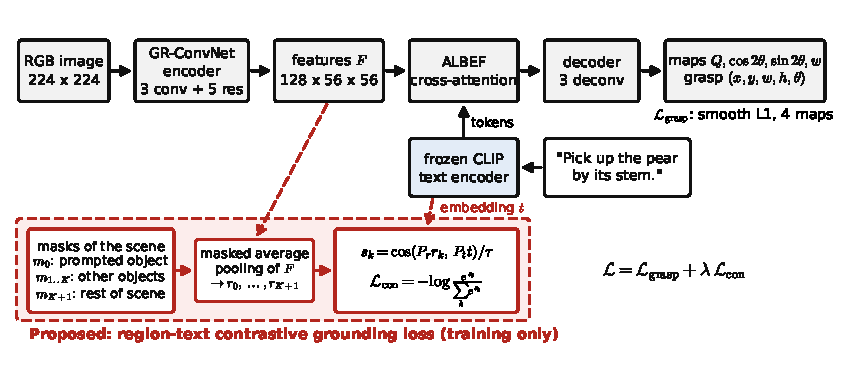
\includegraphics[width=0.92\linewidth]{fig/architecture.pdf}
  \caption{Top: the reproduced GR-ConvNet + CLIP baseline. Bottom (red, training only): the proposed region-text contrastive grounding loss.}
  \label{fig:arch}
\end{figure*}

\paragraph{Baseline.}
GR-ConvNet~\cite{kumra2020antipodal} encodes the $224 \times 224$ image with three convolutions and five residual blocks into features $F \in \mathbb{R}^{128 \times 56 \times 56}$, then decodes four maps: grasp quality $Q$, $\cos 2\theta$, $\sin 2\theta$ and the opening $w$.
The grasp is read at the peak of $Q$.
Following~\cite{vuong2024language}, the prompt is encoded by a frozen CLIP text encoder~\cite{radford2021clip} and fused with the image by an ALBEF-style cross-attention layer~\cite{li2021albef}, in which every position of $F$ attends to the text tokens (\cref{fig:arch}, top).
The paper does not say where the fusion sits; we place it after the encoder, which gives 2.06M parameters, close to the 2.07M reported.
The training loss $\mathcal{L}_{\mathrm{grasp}}$ is the sum of the smooth L1 losses of the four maps.

\paragraph{Region-text contrastive grounding.}
For a prompt about object $0$ of a scene, let $m_0$ be its mask, $m_1, \dots, m_K$ the masks of the other annotated objects, and $m_{K+1} = 1 - \max_k m_k$ the rest of the scene.
We pool the image-only features $F$ (before the fusion) over each region, project the regions and the pooled CLIP embedding $t$ of the prompt with two linear layers $P_r$ and $P_t$, and apply InfoNCE~\cite{oord2018cpc} with object $0$ as the positive:
\begin{equation}
  r_k = \frac{\sum_p m_k(p)\, F(p)}{\sum_p m_k(p)}, \qquad
  s_k = \frac{\cos(P_r r_k,\, P_t t)}{\tau},
  \label{eq:region}
\end{equation}
\begin{equation}
  \mathcal{L}_{\mathrm{con}} = -\log \frac{e^{s_0}}{\sum_{k=0}^{K+1} e^{s_k}}, \qquad
  \mathcal{L} = \mathcal{L}_{\mathrm{grasp}} + \lambda\, \mathcal{L}_{\mathrm{con}}.
  \label{eq:loss}
\end{equation}
The loss gives the encoder the semantic signal its grasp loss lacks: the features of the prompted object must be closer to the prompt than those of objects the robot could grasp by mistake.
The masks of all parts of an object are merged, since the part labels mostly repeat the object label (\cref{sec:experiments}).
$P_r$, $P_t$ and the masks are used in training only, so the inference network is unchanged.
